\documentclass{article}

% content/resources/templates/preamble.tex
\usepackage[margin=0.6in]{geometry}
\author{Milav Dabgar}
\usepackage{amsmath,amssymb,amsthm}
\usepackage{booktabs}
\usepackage{multirow}
\usepackage{xcolor}
\usepackage{tcolorbox}
\tcbuselibrary{breakable,skins}
\usepackage[colorlinks=true,linkcolor=blue]{hyperref}
\usepackage{titlesec}
\usepackage{enumitem}
\usepackage{tikz}
\usepackage{pgfplots}
\usepackage{circuitikz}
\usepackage[version=4]{mhchem}
\usepackage{longtable}
\usepackage{array}
\usepackage{float}
\usepackage{caption}
\usepackage{listings}

\lstset{
  basicstyle=\small\ttfamily,
  breaklines=true,
  breakatwhitespace=false,
  postbreak=\mbox{\textcolor{red}{$\hookrightarrow$}\space},
  float=false,
  numbers=left,
  numberstyle=\tiny\color{gray},
  numbersep=10pt,
  xleftmargin=2em,
  keywordstyle=\color{blue},
  commentstyle=\color{green!60!black},
  stringstyle=\color{purple},
  backgroundcolor=\color{gray!5},
  showstringspaces=false,
  tabsize=2,
  captionpos=b,
  keepspaces=true,
  columns=flexible
}

\pgfplotsset{compat=1.18}
\usetikzlibrary{shapes,arrows,positioning,calc,patterns,decorations.pathmorphing,decorations.markings,arrows.meta}

% Color scheme
\definecolor{headcolor}{RGB}{0,102,204}
\definecolor{keycolor}{RGB}{220,20,60}
\definecolor{solutioncolor}{RGB}{34,139,34}
\definecolor{mnemoniccolor}{RGB}{148,0,211}
\definecolor{codecolor}{RGB}{0,0,100}

% Spacing
\setlength{\parskip}{3pt}
\setlist[itemize]{nosep}
\setlist[enumerate]{nosep}

% Title formatting
\titleformat{\section}{\Large\bfseries\color{headcolor}}{\thesection}{1em}{}
\titleformat{\subsection}{\large\bfseries\color{headcolor}}{\thesubsection}{1em}{}

% Pandoc tightlist compatibility
\providecommand{\tightlist}{%
  \setlength{\itemsep}{0pt}\setlength{\parskip}{0pt}}

% Pandoc longtable compatibility
\newcounter{none}
\def\thenone{}


% content/resources/templates/english-boxes.tex

% Custom environments
\newtcolorbox{solutionbox}{
 breakable,
 enhanced,
 colback=solutioncolor!5!white,
 colframe=solutioncolor!75!black,
 fonttitle=\bfseries,
 title=Solution
}

\newtcolorbox{solutionboxnobreak}{
 colback=solutioncolor!5!white,
 colframe=solutioncolor!75!black,
 fonttitle=\bfseries,
 title=Solution
}

\newtcolorbox{keyformula}{
 breakable,
 enhanced,
 colback=keycolor!5!white,
 colframe=keycolor!75!black,
 fonttitle=\bfseries,
 title=Key Formula
}

\newtcolorbox{mnemonicboxenv}{
 breakable,
 enhanced,
 colback=mnemoniccolor!5!white,
 colframe=mnemoniccolor!75!black,
 fonttitle=\bfseries,
 title=Mnemonic
}

\newcommand{\mnemonicbox}[1]{%
  \begin{mnemonicboxenv}
    #1
  \end{mnemonicboxenv}
}


% Custom commands for GTU solutions
% This file defines semantic commands for consistent formatting

% Question command with automatic formatting
\newcommand{\question}[2]{%
  \section*{Question #1}%
  \textbf{#2}%
}

% OR question variant
\newcommand{\questionor}[2]{%
  \section*{Question #1 OR}%
  \textbf{#2}%
}

% Proper table environment with caption
\newenvironment{answertable}[1]{%
  \begin{table}[htbp]
  \centering
  \caption{#1}
}{%
  \end{table}
}

% Proper figure environment for diagrams
\newenvironment{answerdiagram}[1]{%
  \begin{figure}[htbp]
  \centering
  \caption{#1}
}{%
  \end{figure}
}

% Semantic markup for key terms
\newcommand{\keyword}[1]{\textbf{#1}}
\newcommand{\code}[1]{\texttt{#1}}
\newcommand{\classname}[1]{\texttt{#1}}
\newcommand{\methodname}[1]{\texttt{#1}}

% Proper quotation marks
\newcommand{\mnemonic}[1]{``#1''}


\title{Programming in C (4331105) - Summer 2023 Solution}
\date{July 26, 2023}

\begin{document}
\maketitle

\questionmarks{1}{a}{3}
\textbf{List any six keywords of C language.}

\begin{solutionbox}
    \textbf{Table: Six Keywords in C Language}
    
    \begin{tabulary}{\linewidth}{|L|L|}
        \hline
        \textbf{Keyword} & \textbf{Purpose} \\
        \hline
        \code{int} & Integer data type \\
        \hline
        \code{float} & Floating-point data type \\
        \hline
        \code{if} & Conditional statement \\
        \hline
        \code{while} & Loop structure \\
        \hline
        \code{return} & Returns value from function \\
        \hline
        \code{void} & Specifies empty return type \\
        \hline
    \end{tabulary}

    \begin{mnemonicbox}"I Feel When Running Very Ill" (int, float, while, return, void, if)\end{mnemonicbox}
\end{solutionbox}

\questionmarks{1}{b}{4}
\textbf{Define variable. List the rule for naming of variable in c programming.}

\begin{solutionbox}
    \textbf{Variable}: A named memory location used to store data that can be modified during program execution.

    \textbf{Table: Rules for Variable Naming in C}

    \begin{tabulary}{\linewidth}{|L|L|}
        \hline
        \textbf{Rule} & \textbf{Example} \\
        \hline
        Must begin with letter/underscore & \code{name}, \code{\_value} \\
        \hline
        Can contain letters, digits, underscore & \code{user\_1}, \code{count99} \\
        \hline
        No spaces or special characters & \checkmark: \code{total\_sum}, \ding{55}: \code{total-sum} \\
        \hline
        Case sensitive & \code{Name} $\neq$ \code{name} \\
        \hline
        Cannot use reserved keywords & \ding{55}: \code{int}, \code{while} \\
        \hline
        Maximum 31 characters (standard) & \code{studentRegistrationNumber} \\
        \hline
    \end{tabulary}

    \begin{mnemonicbox}"Letters Lead, No Special Keys" (begins with letter, no special chars, no keywords)\end{mnemonicbox}
\end{solutionbox}

\questionmarks{1}{c}{7}
\textbf{Define flowchart. Draw and Explain flowchart symbols. Write a program to calculate simple interest using below equation. I=PRN/100 Where P=Principal amount, R=Rate of interest and N=Period.}

\begin{solutionbox}
    \textbf{Flowchart}: A graphical representation of an algorithm that uses standard symbols to show the sequence of operations needed to solve a problem.

    \textbf{Table: Flowchart Symbols}

    \begin{tabulary}{\linewidth}{|C|L|L|}
        \hline
        \textbf{Symbol} & \textbf{Name} & \textbf{Purpose} \\
        \hline
        \begin{tikzpicture}
            \node[gtu start, minimum width=2cm, minimum height=1cm] {Start/End};
        \end{tikzpicture} & Terminal & Start/End \\
        \hline
        \begin{tikzpicture}
            \node[gtu process, minimum width=2cm, minimum height=1cm] {Process};
        \end{tikzpicture} & Process & Calculations \\
        \hline
        \begin{tikzpicture}
            \node[gtu input, minimum width=2cm, minimum height=1cm] {Input/Output};
        \end{tikzpicture} & Input/Output & Read/Display data \\
        \hline
        \begin{tikzpicture}
            \node[gtu decision, minimum width=2cm, minimum height=1.5cm] {};
        \end{tikzpicture} & Decision & Conditions \\
        \hline
        $\rightarrow$ & Flow Line & Shows sequence \\
        \hline
    \end{tabulary}

    \textbf{Simple Interest Flowchart:}

    \begin{center}
    \begin{tikzpicture}[gtu flow]
        \node[gtu start] (start) {Start};
        \node[gtu input, below=of start] (input) {Input P, R, N};
        \node[gtu process, below=of input] (calc) {Calculate $I = \frac{P \times R \times N}{100}$};
        \node[gtu input, below=of calc] (disp) {Display I};
        \node[gtu start, below=of disp] (end) {End};

        \draw[gtu arrow] (start) -- (input);
        \draw[gtu arrow] (input) -- (calc);
        \draw[gtu arrow] (calc) -- (disp);
        \draw[gtu arrow] (disp) -- (end);
    \end{tikzpicture}
    \end{center}

    \textbf{Program:}

\begin{lstlisting}[language=C]
#include <stdio.h>
void main()
{
    float p, r, n, i;
    
    printf("Enter principal amount: ");
    scanf("%f", &p);
    
    printf("Enter rate of interest: ");
    scanf("%f", &r);
    
    printf("Enter time period in years: ");
    scanf("%f", &n);
    
    i = (p * r * n) / 100;
    
    printf("Simple Interest = %.2f", i);
}
\end{lstlisting}

    \begin{mnemonicbox}"Please Return Nice Interest" (Principal, Rate, Number of years, Interest)\end{mnemonicbox}
\end{solutionbox}

\questionmarks{1}{c}{7}
\textbf{OR Define algorithm. Write algorithm for finding volume of cylinder. Write a program to read radius(R) and height(H) from user and print calculated the volume(V) of cylinder using. V=$\pi$R$^2$H.}

\begin{solutionbox}
    \textbf{Algorithm}: A step-by-step procedure to solve a problem in a finite amount of time.

    \textbf{Algorithm for Cylinder Volume:}

    \begin{enumerate}
        \item Start
        \item Input radius (R) and height (H)
        \item Calculate volume using formula $V = \pi \times R^2 \times H$
        \item Display the volume
        \item End
    \end{enumerate}

    \textbf{Diagram: Cylinder}

    \begin{center}
    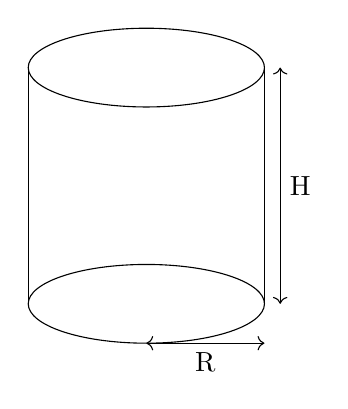
\begin{tikzpicture}
        \draw (0,0) ellipse (1.5 and 0.5);
        \draw (0,3) ellipse (1.5 and 0.5);
        \draw (-1.5,0) -- (-1.5,3);
        \draw (1.5,0) -- (1.5,3);
        
        \draw[<->] (1.7,0) -- (1.7,3) node[midway, right] {H};
        \draw[<->] (0,-0.5) -- (1.5,-0.5) node[midway, below] {R};
    \end{tikzpicture}
    \end{center}

    \textbf{Program:}

\begin{lstlisting}[language=C]
#include <stdio.h>
void main()
{
    float radius, height, volume;
    float pi = 3.14159;
    
    printf("Enter radius of cylinder: ");
    scanf("%f", &radius);
    
    printf("Enter height of cylinder: ");
    scanf("%f", &height);
    
    volume = pi * radius * radius * height;
    
    printf("Volume of cylinder = %.2f", volume);
}
\end{lstlisting}

    \begin{mnemonicbox}"Round Hat Volume" (Radius, Height, Volume)\end{mnemonicbox}
\end{solutionbox}

\questionmarks{2}{a}{3}
\textbf{List out different operators supported in C programming language.}

\begin{solutionbox}
    \textbf{Table: Operators in C Programming}

    \begin{tabulary}{\linewidth}{|L|L|L|}
        \hline
        \textbf{Operator Type} & \textbf{Examples} & \textbf{Use} \\
        \hline
        Arithmetic & +, -, *, /, \% & Mathematical operations \\
        \hline
        Relational & <, >, ==, !=, <=, >= & Compare values \\
        \hline
        Logical & \&\&, ||, ! & Combine conditions \\
        \hline
        Assignment & =, +=, -=, *=, /= & Assign values \\
        \hline
        Increment/Decrement & ++, -- & Increase/decrease by 1 \\
        \hline
        Bitwise & \&, |, \^{}, \~{}, <<, >> & Bit manipulation \\
        \hline
        Conditional & ?: & Short if-else \\
        \hline
    \end{tabulary}

    \begin{mnemonicbox}"All Relationships Lead Ancestors Incrementally Beyond Conditions" (first letter of each type)\end{mnemonicbox}
\end{solutionbox}

\questionmarks{2}{b}{4}
\textbf{Write a program to print sum and average of 1 to 50.}

\begin{solutionbox}
    \textbf{Program:}

\begin{lstlisting}[language=C]
#include <stdio.h>
void main()
{
    int i, sum = 0;
    float avg;
    
    for(i = 1; i <= 50; i++)
    {
        sum = sum + i;
    }
    
    avg = (float)sum / 50;
    
    printf("Sum of numbers from 1 to 50 = %d\n", sum);
    printf("Average of numbers from 1 to 50 = %.2f", avg);
}
\end{lstlisting}

    \textbf{Process Diagram:}

    \begin{center}
    \begin{tikzpicture}[gtu flow]
        \node[gtu start] (start) {Start};
        \node[gtu process, right=of start] (init) {Set sum = 0};
        \node[gtu process, right=of init] (loop) {Loop $i$ from 1 to 50};
        \node[gtu process, below=of loop] (add) {Add $i$ to sum};
        \node[gtu decision, left=of add] (cond) {$i < 50$?};
        \node[gtu process, below=of cond] (calc) {avg = sum/50};
        \node[gtu input, right=of calc] (disp) {Display sum/avg};
        \node[gtu start, right=of disp] (end) {End};

        \draw[gtu arrow] (start) -- (init);
        \draw[gtu arrow] (init) -- (loop);
        \draw[gtu arrow] (loop) -- (add);
        \draw[gtu arrow] (add) -- (cond);
        \draw[gtu arrow] (cond) |- node[near start, right] {Yes} (loop);
        \draw[gtu arrow] (cond) -- node[left] {No} (calc);
        \draw[gtu arrow] (calc) -- (disp);
        \draw[gtu arrow] (disp) -- (end);
    \end{tikzpicture}
    \end{center}

    \begin{mnemonicbox}"Summing And Dividing" (Sum, Average, Division)\end{mnemonicbox}
\end{solutionbox}

\questionmarks{2}{c}{7}
\textbf{Explain arithmetic \& relational operators with example.}

\begin{solutionbox}
    \textbf{Arithmetic Operators:}

    \textbf{Table: Arithmetic Operators in C}

    \begin{tabulary}{\linewidth}{|C|L|L|C|}
        \hline
        \textbf{Operator} & \textbf{Operation} & \textbf{Example} & \textbf{Result} \\
        \hline
        + & Addition & 5 + 3 & 8 \\
        \hline
        - & Subtraction & 7 - 2 & 5 \\
        \hline
        * & Multiplication & 4 * 3 & 12 \\
        \hline
        / & Division & 8 / 4 & 2 \\
        \hline
        \% & Modulus (Remainder) & 7 \% 3 & 1 \\
        \hline
    \end{tabulary}

    \textbf{Relational Operators:}

    \textbf{Table: Relational Operators in C}

    \begin{tabulary}{\linewidth}{|C|L|L|C|}
        \hline
        \textbf{Operator} & \textbf{Meaning} & \textbf{Example} & \textbf{Result} \\
        \hline
        < & Less than & 5 < 8 & 1 (true) \\
        \hline
        > & Greater than & 9 > 3 & 1 (true) \\
        \hline
        == & Equal to & 4 == 4 & 1 (true) \\
        \hline
        != & Not equal to & 7 != 3 & 1 (true) \\
        \hline
        <= & Less than/equal & 4 <= 4 & 1 (true) \\
        \hline
        >= & Greater than/equal & 6 >= 9 & 0 (false) \\
        \hline
    \end{tabulary}

    \textbf{Code Example:}

\begin{lstlisting}[language=C]
#include <stdio.h>
void main()
{
    int a = 10, b = 5;
    
    // Arithmetic operators
    printf("a + b = %d\n", a + b);   // 15
    printf("a - b = %d\n", a - b);   // 5
    printf("a * b = %d\n", a * b);   // 50
    printf("a / b = %d\n", a / b);   // 2
    printf("a %% b = %d\n", a % b);  // 0
    
    // Relational operators
    printf("a < b: %d\n", a < b);    // 0 (false)
    printf("a > b: %d\n", a > b);    // 1 (true)
    printf("a == b: %d\n", a == b);  // 0 (false)
    printf("a != b: %d\n", a != b);  // 1 (true)
}
\end{lstlisting}

    \begin{mnemonicbox}"Add Subtract Multiply Divide Remainder" (arithmetic), "Less Greater Equal Not" (relational)\end{mnemonicbox}
\end{solutionbox}

\questionmarks{2}{a}{3}
\textbf{OR State the difference between gets(S) and scanf("\%s",S) where S is string.}

\begin{solutionbox}
    \textbf{Table: Difference between gets(S) and scanf("\%s",S)}

    \begin{tabulary}{\linewidth}{|L|L|L|}
        \hline
        \textbf{Feature} & \textbf{gets(S)} & \textbf{scanf("\%s",S)} \\
        \hline
        Space handling & Reads spaces between words & Stops reading at space \\
        \hline
        Input termination & Ends at newline character & Ends at whitespace \\
        \hline
        Buffer overflow & Unsafe, no length check & Safer with width limit \\
        \hline
        Example behavior & "Hello World" $\rightarrow$ "Hello World" & "Hello World" $\rightarrow$ "Hello" \\
        \hline
        Security & Deprecated due to overflow risks & Better with width specifier \\
        \hline
    \end{tabulary}

    \begin{mnemonicbox}"Gets Spaces, Scanf Stops" (gets reads spaces, scanf stops at spaces)\end{mnemonicbox}
\end{solutionbox}

\questionmarks{2}{b}{4}
\textbf{OR Write a program to swap two numbers.}

\begin{solutionbox}
    \textbf{Program:}

\begin{lstlisting}[language=C]
#include <stdio.h>
void main()
{
    int a, b, temp;
    
    printf("Enter value of a: ");
    scanf("%d", &a);
    
    printf("Enter value of b: ");
    scanf("%d", &b);
    
    printf("Before swapping: a = %d, b = %d\n", a, b);
    
    // Swapping using temp variable
    temp = a;
    a = b;
    b = temp;
    
    printf("After swapping: a = %d, b = %d", a, b);
}
\end{lstlisting}

    \textbf{Swapping Diagram:}

    \begin{center}
    \begin{tikzpicture}[gtu flow]
        \node[gtu process] (a) {a = 5};
        \node[gtu process, below=of a] (b) {b = 10};
        \node[gtu process, right=of a, xshift=2cm] (temp) {temp = 5};
        \node[gtu process, below=of temp] (a_new) {a = 10};
        \node[gtu process, below=of a_new] (b_new) {b = 5};

        \draw[gtu arrow] (a) -- node[above] {temp = a} (temp);
        \draw[gtu arrow] (b) -- node[above, sloped] {a = b} (a_new);
        \draw[gtu arrow] (temp) -- node[right] {b = temp} (b_new);
    \end{tikzpicture}
    \end{center}

    \begin{mnemonicbox}"Temporary Assists Swapping" (Temp variable enables swapping)\end{mnemonicbox}
\end{solutionbox}

\questionmarks{2}{c}{7}
\textbf{OR Explain Logical operator and bit-wise operator with example.}

\begin{solutionbox}
    \textbf{Logical Operators:}

    \textbf{Table: Logical Operators in C}

    \begin{tabulary}{\linewidth}{|C|L|L|C|}
        \hline
        \textbf{Operator} & \textbf{Description} & \textbf{Example} & \textbf{Result} \\
        \hline
        \&\& & Logical AND & (5>3) \&\& (8>6) & 1 (both true) \\
        \hline
        || & Logical OR & (5<3) || (8>6) & 1 (one true) \\
        \hline
        ! & Logical NOT & !(5>3) & 0 (inverts true) \\
        \hline
    \end{tabulary}

    \textbf{Bitwise Operators:}

    \textbf{Table: Bitwise Operators in C}

    \begin{tabulary}{\linewidth}{|C|L|L|L|}
        \hline
        \textbf{Operator} & \textbf{Description} & \textbf{Example} & \textbf{Binary Result} \\
        \hline
        \& & Bitwise AND & 5 \& 3 & 101 \& 011 = 001 (1) \\
        \hline
        | & Bitwise OR & 5 | 3 & 101 | 011 = 111 (7) \\
        \hline
        \^{} & Bitwise XOR & 5 \^{} 3 & 101 \^{} 011 = 110 (6) \\
        \hline
        \~{} & Bitwise NOT & \~{}5 & \~{}0101 = 1010 (-6) \\
        \hline
        << & Left Shift & 5 << 1 & 101 << 1 = 1010 (10) \\
        \hline
        >> & Right Shift & 5 >> 1 & 101 >> 1 = 10 (2) \\
        \hline
    \end{tabulary}

    \textbf{Code Example:}

\begin{lstlisting}[language=C]
#include <stdio.h>
void main()
{
    int a = 5, b = 3;
    
    // Logical operators
    printf("a>3 && b<5: %d\n", (a>3) && (b<5));  // 1 (true)
    printf("a<3 || b>1: %d\n", (a<3) || (b>1));  // 1 (true)
    printf("!(a>b): %d\n", !(a>b));              // 0 (false)
    
    // Bitwise operators
    printf("a & b: %d\n", a & b);   // 1
    printf("a | b: %d\n", a | b);   // 7
    printf("a ^ b: %d\n", a ^ b);   // 6
    printf("~a: %d\n", ~a);         // -6
    printf("a << 1: %d\n", a << 1); // 10
    printf("a >> 1: %d\n", a >> 1); // 2
}
\end{lstlisting}

    \begin{mnemonicbox}"AND OR NOT" (logical), "AND OR XOR NOT SHIFT" (bitwise)\end{mnemonicbox}
\end{solutionbox}

\questionmarks{3}{a}{3}
\textbf{Explain multiple if-else statement with example.}

\begin{solutionbox}
    \textbf{Multiple if-else}: Series of if-else statements where each condition is checked sequentially until a true condition is found.

    \textbf{Structure:}

\begin{lstlisting}[language=C]
if (condition1)
    statement1;
else if (condition2)
    statement2;
else if (condition3)
    statement3;
else
    default_statement;
\end{lstlisting}

    \textbf{Code Example:}

\begin{lstlisting}[language=C]
#include <stdio.h>
void main()
{
    int marks;
    
    printf("Enter marks: ");
    scanf("%d", &marks);
    
    if (marks >= 80)
        printf("Grade: A");
    else if (marks >= 70)
        printf("Grade: B");
    else if (marks >= 60)
        printf("Grade: C");
    else if (marks >= 50)
        printf("Grade: D");
    else
        printf("Grade: F");
}
\end{lstlisting}

    \textbf{Diagram:}

    \begin{center}
    \begin{tikzpicture}[gtu flow]
        \node[gtu start] (start) {Start};
        \node[gtu decision, alias=d1, below=of start] {marks $\ge$ 80?};
        \node[gtu process, right=of d1] (g1) {Grade A};
        \node[gtu decision, alias=d2, below=of d1] {marks $\ge$ 70?};
        \node[gtu process, right=of d2] (g2) {Grade B};
        \node[gtu decision, alias=d3, below=of d2] {marks $\ge$ 60?};
        \node[gtu process, right=of d3] (g3) {Grade C};
        \node[gtu decision, alias=d4, below=of d3] {marks $\ge$ 50?};
        \node[gtu process, right=of d4] (g4) {Grade D};
        \node[gtu process, below=of d4] (g5) {Grade F};
        
        \draw[gtu arrow] (start) -- (d1);
        \draw[gtu arrow] (d1) -- node[above] {Yes} (g1);
        \draw[gtu arrow] (d1) -- node[left] {No} (d2);
        \draw[gtu arrow] (d2) -- node[above] {Yes} (g2);
        \draw[gtu arrow] (d2) -- node[left] {No} (d3);
        \draw[gtu arrow] (d3) -- node[above] {Yes} (g3);
        \draw[gtu arrow] (d3) -- node[left] {No} (d4);
        \draw[gtu arrow] (d4) -- node[above] {Yes} (g4);
        \draw[gtu arrow] (d4) -- node[left] {No} (g5);
    \end{tikzpicture}
    \end{center}

    \begin{mnemonicbox}"Check Each Condition in Sequence" (CECS)\end{mnemonicbox}
\end{solutionbox}

\questionmarks{3}{b}{4}
\textbf{State the working of while loop and for loop.}

\begin{solutionbox}
    \textbf{Table: While Loop vs For Loop}

    \begin{tabulary}{\linewidth}{|L|L|L|}
        \hline
        \textbf{Feature} & \textbf{While Loop} & \textbf{For Loop} \\
        \hline
        Syntax & \code{while(cond) \{ stmt; \}} & \code{for(init; cond; upd) \{ stmt; \}} \\
        \hline
        When to use & Iterations unknown & Iterations known \\
        \hline
        Initialization & Before loop & Inside declaration \\
        \hline
        Update & Inside loop body & In declaration \\
        \hline
        Exit control & Beginning & Beginning \\
        \hline
        Example & User input check & Fixed count \\
        \hline
    \end{tabulary}

    \begin{minipage}{0.45\textwidth}
    \textbf{While Loop Flow:}
    \begin{center}
    \begin{tikzpicture}[gtu flow, scale=0.7, transform shape]
        \node[gtu start] (start) {Start};
        \node[gtu process, below=of start] (init) {Init};
        \node[gtu decision, below=of init] (cond) {Cond};
        \node[gtu process, right=of cond] (body) {Body};
        \node[gtu start, below=of cond] (end) {End};

        \draw[gtu arrow] (start) -- (init);
        \draw[gtu arrow] (init) -- (cond);
        \draw[gtu arrow] (cond) -- node[above] {True} (body);
        \draw[gtu arrow] (body) |- (cond);
        \draw[gtu arrow] (cond) -- node[left] {False} (end);
    \end{tikzpicture}
    \end{center}
    \end{minipage}
    \hfill
    \begin{minipage}{0.45\textwidth}
    \textbf{For Loop Flow:}
    \begin{center}
    \begin{tikzpicture}[gtu flow, scale=0.7, transform shape]
        \node[gtu start] (start) {Start};
        \node[gtu process, below=of start] (init) {Init};
        \node[gtu decision, below=of init] (cond) {Cond};
        \node[gtu process, right=of cond] (body) {Body};
        \node[gtu process, below=of body] (upd) {Update};
        \node[gtu start, below=of cond] (end) {End};

        \draw[gtu arrow] (start) -- (init);
        \draw[gtu arrow] (init) -- (cond);
        \draw[gtu arrow] (cond) -- node[above] {True} (body);
        \draw[gtu arrow] (body) -- (upd);
        \draw[gtu arrow] (upd) |- (cond);
        \draw[gtu arrow] (cond) -- node[left] {False} (end);
    \end{tikzpicture}
    \end{center}
    \end{minipage}

    \begin{mnemonicbox}"While Checks Then Acts" (WCTA), "For Initializes Tests Updates" (FITU)\end{mnemonicbox}
\end{solutionbox}

\questionmarks{3}{c}{7}
\textbf{Write a program to find factorial of a given number.}

\begin{solutionbox}
    \textbf{Program:}

\begin{lstlisting}[language=C]
#include <stdio.h>
void main()
{
    int num, i;
    unsigned long fact = 1;
    
    printf("Enter a number: ");
    scanf("%d", &num);
    
    if (num < 0)
        printf("Factorial not defined for negative numbers");
    else
    {
        for(i = 1; i <= num; i++)
        {
            fact = fact * i;
        }
        printf("Factorial of %d = %lu", num, fact);
    }
}
\end{lstlisting}

    \textbf{Factorial Calculation Table:}
    For example, if num = 5:

    \begin{tabulary}{\linewidth}{|C|C|L|C|}
        \hline
        \textbf{Iter} & \textbf{i} & \textbf{fact * i} & \textbf{New fact} \\
        \hline
        Init & - & - & 1 \\
        \hline
        1 & 1 & 1 * 1 & 1 \\
        \hline
        2 & 2 & 1 * 2 & 2 \\
        \hline
        3 & 3 & 2 * 3 & 6 \\
        \hline
        4 & 4 & 6 * 4 & 24 \\
        \hline
        5 & 5 & 24 * 5 & 120 \\
        \hline
    \end{tabulary}

    \textbf{Factorial Calculation Diagram:}

    \begin{center}
    \begin{tikzpicture}[gtu flow]
        \node[gtu start] (start) {Start};
        \node[gtu input, below=of start] (inp) {Input num};
        \node[gtu decision, below=of inp] (chk) {num < 0?};
        \node[gtu process, right=of chk] (err) {Error};
        \node[gtu process, below=of chk] (init) {fact = 1};
        \node[gtu process, below=of init] (loop) {Loop $i=1$ to $num$};
        \node[gtu process, below=of loop] (calc) {fact *= i};
        \node[gtu decision, below=of calc] (lchk) {More $i$?};
        \node[gtu input, below=of lchk] (disp) {Display fact};
        \node[gtu start, below=of disp] (end) {End};

        \draw[gtu arrow] (start) -- (inp);
        \draw[gtu arrow] (inp) -- (chk);
        \draw[gtu arrow] (chk) -- node[above] {Yes} (err);
        \draw[gtu arrow] (chk) -- node[left] {No} (init);
        \draw[gtu arrow] (init) -- (loop);
        \draw[gtu arrow] (loop) -- (calc);
        \draw[gtu arrow] (calc) -- (lchk);
        \draw[gtu arrow] (lchk) -- node[right] {No} (disp);
        \draw[gtu arrow] (lchk.east) -- ++(0.5,0) |- (loop.east);
        \draw[gtu arrow] (disp) -- (end);
    \end{tikzpicture}
    \end{center}

    \begin{mnemonicbox}"Find And Count The Numbers!" (FACTN! - Factorial)\end{mnemonicbox}
\end{solutionbox}

\questionmarks{3}{a}{3}
\textbf{OR Explain the working of switch-case statement with example.}

\begin{solutionbox}
    \textbf{Switch-Case}: A selection statement that allows a variable to be tested for equality against a list of values (cases).

    \textbf{Structure:}

\begin{lstlisting}[language=C]
switch(expression) {
    case value1:
        statements1;
        break;
    case value2:
        statements2;
        break;
    default:
        default_statements;
}
\end{lstlisting}

    \textbf{Code Example:}

\begin{lstlisting}[language=C]
#include <stdio.h>
void main()
{
    int day;
    printf("Enter day number (1-7): ");
    scanf("%d", &day);
    
    switch(day) {
        case 1: printf("Monday"); break;
        case 2: printf("Tuesday"); break;
        case 3: printf("Wednesday"); break;
        case 4: printf("Thursday"); break;
        case 5: printf("Friday"); break;
        case 6: printf("Saturday"); break;
        case 7: printf("Sunday"); break;
        default: printf("Invalid day");
    }
}
\end{lstlisting}

    \begin{mnemonicbox}"Select Value, Exit with Break" (SVEB)\end{mnemonicbox}
\end{solutionbox}

\questionmarks{3}{b}{4}
\textbf{OR State the use of break and continue keyword.}

\begin{solutionbox}
    \textbf{Table: Break vs Continue Keywords}

    \begin{tabulary}{\linewidth}{|L|L|L|}
        \hline
        \textbf{Feature} & \textbf{break} & \textbf{continue} \\
        \hline
        Purpose & Exits loop/switch & Skips iteration \\
        \hline
        Effect & Terminates loop & Next iteration \\
        \hline
        Where used & Loops \& switch & Loops only \\
        \hline
        Flow & After loop & Condition check \\
        \hline
    \end{tabulary}

    \textbf{Flow Diagram - break:}

    \begin{center}
    \begin{tikzpicture}[gtu flow]
        \node[gtu start] (start) {Start};
        \node[gtu process, right=of start] (loop) {Loop};
        \node[gtu decision, right=of loop] (cond) {Cond?};
        \node[gtu process, below=of cond] (break) {break};
        \node[gtu start, right=of cond] (endloop) {Rest of loop};
        \node[gtu start, below=of break] (end) {End};

        \draw[gtu arrow] (start) -- (loop);
        \draw[gtu arrow] (loop) -- (cond);
        \draw[gtu arrow] (cond) -- node[left] {True} (break);
        \draw[gtu arrow] (cond) -- node[above] {False} (endloop);
        \draw[gtu arrow] (break) -- (end);
        \draw[gtu arrow] (endloop) |- (loop);
    \end{tikzpicture}
    \end{center}

    \begin{mnemonicbox}"Break Exits, Continue Skips" (BECS)\end{mnemonicbox}
\end{solutionbox}

\questionmarks{3}{c}{7}
\textbf{OR Write a program to read number of lines (n) from keyboard and print the triangle shown below. For Example, n=5}

\begin{solutionbox}
    \textbf{Target Pattern:}
    
\begin{verbatim}
1 2 3 4 5
1 2 3 4
1 2 3
1 2
1
\end{verbatim}

    \textbf{Program:}

\begin{lstlisting}[language=C]
#include <stdio.h>
void main()
{
    int n, i, j;
    
    printf("Enter number of lines: ");
    scanf("%d", &n);
    
    for(i = n; i >= 1; i--)
    {
        for(j = 1; j <= i; j++)
        {
            printf("%d ", j);
        }
        printf("\n");
    }
}
\end{lstlisting}

    \textbf{Pattern Logic Table:}
    For n = 5:

    \begin{tabulary}{\linewidth}{|C|C|L|}
        \hline
        \textbf{i} & \textbf{j range} & \textbf{Output} \\
        \hline
        5 & 1 to 5 & 1 2 3 4 5 \\
        \hline
        4 & 1 to 4 & 1 2 3 4 \\
        \hline
        3 & 1 to 3 & 1 2 3 \\
        \hline
        2 & 1 to 2 & 1 2 \\
        \hline
        1 & 1 to 1 & 1 \\
        \hline
    \end{tabulary}

    \begin{mnemonicbox}"Decreasing Rows With Increasing Values" (DRWIV)\end{mnemonicbox}
\end{solutionbox}

\questionmarks{4}{a}{3}
\textbf{Explain nested if-else statement with example.}

\begin{solutionbox}
    \textbf{Nested if-else}: An if-else statement inside another if or else block.

    \textbf{Structure:}

\begin{lstlisting}[language=C]
if (condition1) {
    if (condition2) {
        statements1;
    } else {
        statements2;
    }
} else {
    statements3;
}
\end{lstlisting}

    \textbf{Code Example:}

\begin{lstlisting}[language=C]
#include <stdio.h>
void main()
{
    int age, weight;
    
    printf("Enter age: ");
    scanf("%d", &age);
    
    if (age >= 18) {
        printf("Enter weight: ");
        scanf("%d", &weight);
        
        if (weight >= 50) {
            printf("Eligible to donate blood");
        } else {
            printf("Underweight, not eligible");
        }
    } else {
        printf("Age below 18, not eligible");
    }
}
\end{lstlisting}

    \textbf{Nested if-else Diagram:}

    \begin{center}
    \begin{tikzpicture}[gtu flow]
        \node[gtu start] (start) {Start};
        \node[gtu decision, alias=d1, below=of start] {age $\ge$ 18?};
        \node[gtu decision, alias=d2, right=of d1, xshift=2cm] {weight $\ge$ 50?};
        \node[gtu process, below=of d1] (not_age) {Not eligible: Age};
        \node[gtu process, right=of d2] (eligible) {Eligible};
        \node[gtu process, below=of d2] (not_weight) {Not eligible: Weight};
        \node[gtu start, below=of not_weight] (end) {End};

        \draw[gtu arrow] (start) -- (d1);
        \draw[gtu arrow] (d1) -- node[above] {Yes} (d2);
        \draw[gtu arrow] (d1) -- node[left] {No} (not_age);
        \draw[gtu arrow] (d2) -- node[above] {Yes} (eligible);
        \draw[gtu arrow] (d2) -- node[left] {No} (not_weight);
        
        \draw[gtu arrow] (not_age) |- (end);
        \draw[gtu arrow] (not_weight) -- (end);
        \draw[gtu arrow] (eligible) |- (end);
    \end{tikzpicture}
    \end{center}

    \begin{mnemonicbox}"Check Outside Then Inside" (COTI)\end{mnemonicbox}
\end{solutionbox}

\questionmarks{4}{b}{4}
\textbf{Write a program to exchange two integer numbers using pointer arguments.}

\begin{solutionbox}
    \textbf{Program:}

\begin{lstlisting}[language=C]
#include <stdio.h>
void main()
{
    int a, b, temp;
    int *p1, *p2;
    
    printf("Enter value of a: ");
    scanf("%d", &a);
    
    printf("Enter value of b: ");
    scanf("%d", &b);
    
    p1 = &a;  // p1 points to a
    p2 = &b;  // p2 points to b
    
    printf("Before swapping: a = %d, b = %d\n", a, b);
    
    // Swapping using pointers
    temp = *p1;
    *p1 = *p2;
    *p2 = temp;
    
    printf("After swapping: a = %d, b = %d", a, b);
}
\end{lstlisting}

    \textbf{Pointer Swapping Diagram:}

    \begin{center}
    \begin{tikzpicture}
        \node[draw, minimum size=1cm] (a) {5};
        \node[draw, minimum size=1cm, below=of a] (b) {10};
        \node[left=0.2cm of a] {a};
        \node[left=0.2cm of b] {b};
        
        \node[draw, minimum size=1cm, right=2cm of a] (p1) {addr(a)};
        \node[draw, minimum size=1cm, right=2cm of b] (p2) {addr(b)};
        \node[right=0.2cm of p1] {p1};
        \node[right=0.2cm of p2] {p2};
        
        \draw[->, thick, shorten >=2pt] (p1) -- (a);
        \draw[->, thick, shorten >=2pt] (p2) -- (b);
        
        \node[below=1.5cm of b] (text) {After swapping values via pointers:};
        
        \node[draw, minimum size=1cm, below=0.5cm of text] (a2) {10};
        \node[draw, minimum size=1cm, below=of a2] (b2) {5};
        \node[left=0.2cm of a2] {a};
        \node[left=0.2cm of b2] {b};
    \end{tikzpicture}
    \end{center}

    \begin{mnemonicbox}"Pointers Exchange Memory Values" (PEMV)\end{mnemonicbox}
\end{solutionbox}

\questionmarks{4}{c}{7}
\textbf{Define Array. Explain initialization \& declaration of one-dimensional array.}

\begin{solutionbox}
    \textbf{Array}: A collection of elements of the same data type stored in contiguous memory locations and accessed using indices.

    \textbf{Table: Array Declaration \& Initialization}

    \begin{tabulary}{\linewidth}{|L|L|L|}
        \hline
        \textbf{Operation} & \textbf{Syntax} & \textbf{Example} \\
        \hline
        Declaration & \code{type name[size];} & \code{int marks[5];} \\
        \hline
        Init at decl & \code{type name[size] = \{vals\};} & \code{int nums[4] = \{10, 20\};} \\
        \hline
        Partial init & \code{type name[size] = \{vals\};} & \code{int nums[5] = \{10\};} \\
        \hline
        No size & \code{type name[] = \{vals\};} & \code{int nums[] = \{1, 2\};} \\
        \hline
        Individual & \code{name[index] = value;} & \code{marks[0] = 95;} \\
        \hline
    \end{tabulary}

    \textbf{Code Example:}

\begin{lstlisting}[language=C]
#include <stdio.h>
void main()
{
    // Declaration
    int marks[5];
    
    // Initialization after declaration
    marks[0] = 85; marks[1] = 90;
    marks[2] = 78; marks[3] = 92; marks[4] = 88;
    
    // Declaration with initialization
    int scores[] = {95, 89, 76, 82, 91};
    
    printf("marks[2] = %d\n", marks[2]);
}
\end{lstlisting}

    \textbf{Memory Representation:}

    \begin{center}
    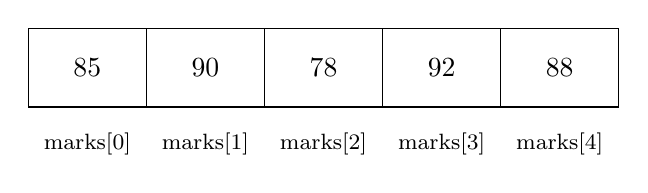
\begin{tikzpicture}
        \foreach \x/\val in {0/85, 1/90, 2/78, 3/92, 4/88} {
            \node[draw, minimum width=1.5cm, minimum height=1cm] at (\x*1.5, 0) (box\x) {\val};
            \node[below=0.2cm of box\x] {\footnotesize marks[\x]};
        }
    \end{tikzpicture}
    \end{center}

    \begin{mnemonicbox}"Declare, Initialize, Access With Index" (DIAWI)\end{mnemonicbox}
\end{solutionbox}

\questionmarks{4}{a}{3}
\textbf{OR Explain do while loop with example.}

\begin{solutionbox}
    \textbf{do-while loop}: A loop that executes the body at least once before checking the condition.

    \textbf{Structure:}

\begin{lstlisting}[language=C]
do {
    statements;
} while(condition);
\end{lstlisting}

    \textbf{Code Example:}

\begin{lstlisting}[language=C]
#include <stdio.h>
void main()
{
    int num, sum = 0;
    do {
        printf("Enter a number (0 to stop): ");
        scanf("%d", &num);
        sum += num;
    } while(num != 0);
    printf("Sum = %d", sum);
}
\end{lstlisting}

    \textbf{do-while Loop Flow:}

    \begin{center}
    \begin{tikzpicture}[gtu flow]
        \node[gtu start] (start) {Start};
        \node[gtu process, below=of start] (body) {Body statements};
        \node[gtu decision, below=of body] (cond) {Condition?};
        \node[gtu start, below=of cond] (end) {End};

        \draw[gtu arrow] (start) -- (body);
        \draw[gtu arrow] (body) -- (cond);
        \draw[gtu arrow] (cond) -- node[left] {False} (end);
        \draw[gtu arrow] (cond.east) -- ++(0.5,0) |- node[near start, right] {True} (body.east);
    \end{tikzpicture}
    \end{center}

    \textbf{Key Differences from while loop:}
    \begin{itemize}
        \item Body executes at least once
        \item Condition checked after execution
        \item Semicolon required after condition
    \end{itemize}

    \begin{mnemonicbox}"Do First, Check Later" (DFCL)\end{mnemonicbox}
\end{solutionbox}

\questionmarks{4}{b}{4}
\textbf{OR Explain following functions with example: (1) gets() (2) puts() (3) strlen() (4) strcpy()}

\begin{solutionbox}
    \textbf{Table: String Functions in C}

    \begin{tabulary}{\linewidth}{|L|L|L|}
        \hline
        \textbf{Function} & \textbf{Purpose} & \textbf{Example} \\
        \hline
        gets() & Reads string with spaces & \code{gets(name);} \\
        \hline
        puts() & Displays string + newline & \code{puts(name);} \\
        \hline
        strlen() & Returns string length & \code{n = strlen(str);} \\
        \hline
        strcpy() & Copies src to dest & \code{strcpy(d, s);} \\
        \hline
    \end{tabulary}

    \textbf{Code Example:}

\begin{lstlisting}[language=C]
#include <stdio.h>
#include <string.h>
void main()
{
    char name[50], copy[50];
    int length;
    
    printf("Enter name: ");
    gets(name);           
    puts(name);
    
    length = strlen(name);
    printf("Length: %d\n", length);
    
    strcpy(copy, name);
    printf("Copied: %s", copy);
}
\end{lstlisting}

    \begin{mnemonicbox}"Gets Puts String's Length and Copies" (GPSLC)\end{mnemonicbox}
\end{solutionbox}

\questionmarks{4}{c}{7}
\textbf{OR Define recursion and explain with suitable example. Write a program to find factorial of a given number using recursion.}

\begin{solutionbox}
    \textbf{Recursion}: A process where a function calls itself directly or indirectly until a specific condition is met.

    \textbf{Components}:
    \begin{enumerate}
        \item Base case: Condition to stop recursion.
        \item Recursive case: Function calling itself.
    \end{enumerate}

    \textbf{Code Example:}

\begin{lstlisting}[language=C]
#include <stdio.h>

unsigned long factorial(int n)
{
    if (n <= 1)
        return 1;
    else
        return n * factorial(n-1);
}

void main()
{
    int num;
    printf("Enter a number: ");
    scanf("%d", &num);
    printf("Factorial of %d = %lu", num, factorial(num));
}
\end{lstlisting}

    \textbf{Recursion Trace for factorial(5):}

    \begin{tabulary}{\linewidth}{|L|L|L|}
        \hline
        \textbf{Call} & \textbf{Step} & \textbf{Result} \\
        \hline
        fact(5) & $5 \times$ fact(4) & $5 \times 24 = 120$ \\
        \hline
        fact(4) & $4 \times$ fact(3) & $4 \times 6 = 24$ \\
        \hline
        fact(3) & $3 \times$ fact(2) & $3 \times 2 = 6$ \\
        \hline
        fact(2) & $2 \times$ fact(1) & $2 \times 1 = 2$ \\
        \hline
        fact(1) & Base case & 1 \\
        \hline
    \end{tabulary}

    \textbf{Recursion Diagram:}

    \begin{center}
    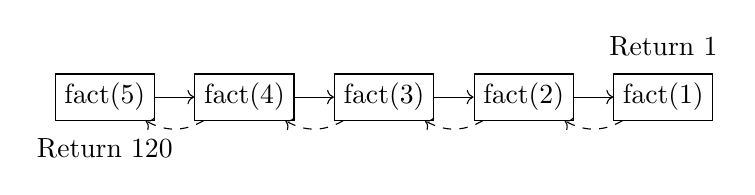
\begin{tikzpicture}
        \node[draw] (f5) {fact(5)};
        \node[draw, right=0.5cm of f5] (f4) {fact(4)};
        \node[draw, right=0.5cm of f4] (f3) {fact(3)};
        \node[draw, right=0.5cm of f3] (f2) {fact(2)};
        \node[draw, right=0.5cm of f2] (f1) {fact(1)};

        \draw[->] (f5) -- (f4);
        \draw[->] (f4) -- (f3);
        \draw[->] (f3) -- (f2);
        \draw[->] (f2) -- (f1);
        \draw[->, dashed] (f1) to[bend left] (f2);
        \draw[->, dashed] (f2) to[bend left] (f3);
        \draw[->, dashed] (f3) to[bend left] (f4);
        \draw[->, dashed] (f4) to[bend left] (f5);
        
        \node[above=0.1cm of f1] {Return 1};
        \node[below=0.1cm of f5] {Return 120};
    \end{tikzpicture}
    \end{center}

    \begin{mnemonicbox}"Function Calling Itself, Bottoming Out" (FCIBO)\end{mnemonicbox}
\end{solutionbox}

\questionmarks{5}{a}{3}
\textbf{Write the difference between array and structure.}

\begin{solutionbox}
    \textbf{Table: Array vs Structure}

    \begin{tabulary}{\linewidth}{|L|L|L|}
        \hline
        \textbf{Feature} & \textbf{Array} & \textbf{Structure} \\
        \hline
        Data type & Same for all elements & Different types \\
        \hline
        Access & Index (\code{arr[0]}) & Member (\code{s.name}) \\
        \hline
        Memory & Contiguous & Contiguous (mixed) \\
        \hline
        Size & Fixed & Sum of members \\
        \hline
        Purpose & Collection of similar & Grouping related \\
        \hline
        Decl & \code{int a[5];} & \code{struct s \{ int a; \};} \\
        \hline
    \end{tabulary}

    \textbf{Diagram:}

    \begin{center}
    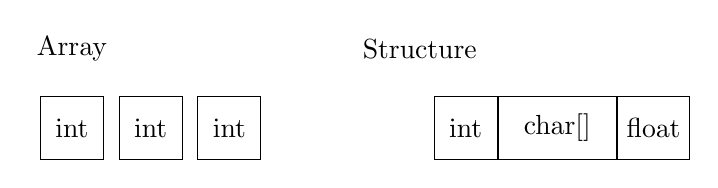
\begin{tikzpicture}
        \node (arr) {Array};
        \foreach \x in {0,1,2} {
            \node[draw, minimum size=0.8cm] at (\x, -1) (a\x) {int};
        }
        
        \node[right=3cm of arr] (str) {Structure};
        \node[draw, minimum width=0.8cm, minimum height=0.8cm] at (5, -1) (s1) {int};
        \node[draw, minimum width=1.5cm, minimum height=0.8cm, right=0cm of s1] (s2) {char[]};
        \node[draw, minimum width=0.8cm, minimum height=0.8cm, right=0cm of s2] (s3) {float};
    \end{tikzpicture}
    \end{center}

    \begin{mnemonicbox}"Arrays for Same, Structures for Different" (ASSD)\end{mnemonicbox}
\end{solutionbox}

\questionmarks{5}{b}{4}
\textbf{Write a C program using array that find the maximum value from given 10 values.}

\begin{solutionbox}
    \textbf{Program:}

\begin{lstlisting}[language=C]
#include <stdio.h>
void main()
{
    int arr[10], i, max;
    
    printf("Enter 10 values:\n");
    for(i = 0; i < 10; i++) {
        scanf("%d", &arr[i]);
    }
    
    max = arr[0]; 
    for(i = 1; i < 10; i++) {
        if(arr[i] > max)
            max = arr[i];
    }
    
    printf("Maximum value is: %d", max);
}
\end{lstlisting}

    \textbf{Algorithm Flow:}

    \begin{center}
    \begin{tikzpicture}[gtu flow]
        \node[gtu start] (start) {Start};
        \node[gtu input, below=of start] (input) {Input 10 values};
        \node[gtu process, below=of input] (init) {max = arr[0]};
        \node[gtu process, right=of init] (loop) {Loop $i=1$ to 9};
        \node[gtu decision, right=of loop] (check) {arr[i] > max?};
        \node[gtu process, below=of check] (update) {max = arr[i]};
        \node[gtu input, below=of init] (disp) {Display max};
        \node[gtu start, below=of disp] (end) {End};
        
        \draw[gtu arrow] (start) -- (input);
        \draw[gtu arrow] (input) -- (init);
        \draw[gtu arrow] (init) -- (loop);
        \draw[gtu arrow] (loop) -- (check);
        \draw[gtu arrow] (check) -- node[right] {Yes} (update);
        \draw[gtu arrow] (check) -- node[above] {No} ++(2,0) |- (loop);
        \draw[gtu arrow] (update) -- ++(-1.5,0) |- (loop);
        
        \draw[gtu arrow] (loop) -- node[left] {Done} (disp);
        \draw[gtu arrow] (disp) -- (end);
    \end{tikzpicture}
    \end{center}

    \begin{mnemonicbox}"Compare And Replace Maximum" (CARM)\end{mnemonicbox}
\end{solutionbox}

\questionmarks{5}{c}{7}
\textbf{Define structure? Develop a structure named book to save following information about books. Book title, Name of author, Price and Number of pages.}

\begin{solutionbox}
    \textbf{Structure}: A user-defined data type that groups related variables of different data types under a single name.

    \textbf{Book Structure Code:}

\begin{lstlisting}[language=C]
#include <stdio.h>

struct book {
    char title[50];
    char author[30];
    float price;
    int pages;
};

void main()
{
    struct book b1;
    
    printf("Enter book title: "); gets(b1.title);
    printf("Enter author name: "); gets(b1.author);
    printf("Enter price: "); scanf("%f", &b1.price);
    printf("Enter pages: "); scanf("%d", &b1.pages);
    
    printf("\nBook Details:\n");
    printf("Title: %s\n", b1.title);
    printf("Author: %s\n", b1.author);
    printf("Price: %.2f\n", b1.price);
    printf("Pages: %d", b1.pages);
}
\end{lstlisting}

    \textbf{Structure Diagram:}

    \begin{center}
    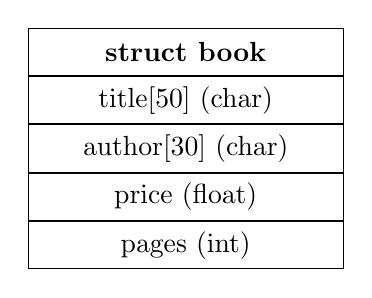
\begin{tikzpicture}
        \node[draw, minimum width=4cm, minimum height=0.6cm] (header) {\textbf{struct book}};
        \node[draw, minimum width=4cm, minimum height=0.6cm, below=0cm of header] (f1) {title[50] (char)};
        \node[draw, minimum width=4cm, minimum height=0.6cm, below=0cm of f1] (f2) {author[30] (char)};
        \node[draw, minimum width=4cm, minimum height=0.6cm, below=0cm of f2] (f3) {price (float)};
        \node[draw, minimum width=4cm, minimum height=0.6cm, below=0cm of f3] (f4) {pages (int)};
    \end{tikzpicture}
    \end{center}

    \begin{mnemonicbox}"Title Author Price Pages" (TAPP)\end{mnemonicbox}
\end{solutionbox}

\questionmarks{5}{a}{3}
\textbf{OR What is a string? What are the operations that can be performed on string?}

\begin{solutionbox}
    \textbf{String}: A sequence of characters terminated by a null character '\textbackslash0'.

    \textbf{Table: String Operations in C}

    \begin{tabulary}{\linewidth}{|L|L|L|}
        \hline
        \textbf{Operation} & \textbf{Function} & \textbf{Example} \\
        \hline
        Input & gets, scanf & \code{gets(s)} \\
        \hline
        Output & puts, printf & \code{puts(s)} \\
        \hline
        Length & strlen & \code{l=strlen(s)} \\
        \hline
        Copy & strcpy & \code{strcpy(d,s)} \\
        \hline
        Concat & strcat & \code{strcat(s1,s2)} \\
        \hline
        Compare & strcmp & \code{strcmp(s1,s2)} \\
        \hline
        Search & strchr & \code{strchr(s,'a')} \\
        \hline
    \end{tabulary}

    \textbf{String Representation:}

    \begin{center}
    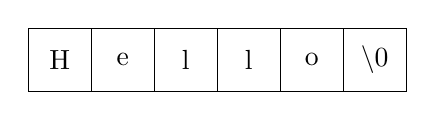
\begin{tikzpicture}
        \foreach \x/\vchar in {0/H, 1/e, 2/l, 3/l, 4/o, 5/\textbackslash 0} {
            \node[draw, minimum size=0.8cm] at (\x*0.8, 0) {\vchar};
        }
    \end{tikzpicture}
    \end{center}

    \begin{mnemonicbox}"Input Output Length Copy Concat Compare Search Convert" (IOLCCSC)\end{mnemonicbox}
\end{solutionbox}

\questionmarks{5}{b}{4}
\textbf{OR Write a program prints its ASCII value from A to Z.}

\begin{solutionbox}
    \textbf{Program:}

\begin{lstlisting}[language=C]
#include <stdio.h>
void main()
{
    char ch;
    
    printf("ASCII values from A to Z:\n");
    printf("Char\tValue\n");
    
    for(ch = 'A'; ch <= 'Z'; ch++)
    {
        printf("%c\t%d\n", ch, ch);
    }
}
\end{lstlisting}

    \textbf{ASCII Representation:}

    \begin{center}
    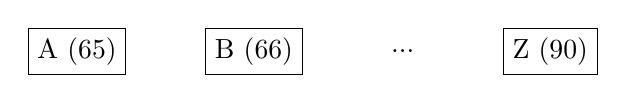
\begin{tikzpicture}
        \node[draw] (a) {A (65)};
        \node[draw, right=of a] (b) {B (66)};
        \node[right=of b] (dots) {...};
        \node[draw, right=of dots] (z) {Z (90)};
    \end{tikzpicture}
    \end{center}

    \begin{mnemonicbox}"Alphabets Sequentially Creating Integer Indices" (ASCII)\end{mnemonicbox}
\end{solutionbox}

\questionmarks{5}{c}{7}
\textbf{OR What is user defined and library function? Explain with two examples of each.}

\begin{solutionbox}
    \textbf{Library Functions}: Pre-defined functions provided by C language that are ready to use (e.g., printf, sqrt).
    \textbf{User-Defined Functions}: Functions created by the programmer to perform specific tasks.

    \textbf{Table: Library vs User-Defined Functions}

    \begin{tabulary}{\linewidth}{|L|L|L|}
        \hline
        \textbf{Feature} & \textbf{Library Functions} & \textbf{User-Defined Functions} \\
        \hline
        Definition & Pre-defined & By programmer \\
        \hline
        Decl & Not needed & Required \\
        \hline
        Header & Required (stdio.h) & Not required \\
        \hline
        Purpose & Common tasks & Custom tasks \\
        \hline
    \end{tabulary}

    \textbf{Examples:}
    
    1. \textbf{Library}: \code{strlen("Hi")} (string.h), \code{sqrt(25)} (math.h)
    
    2. \textbf{User-Defined}:
\begin{lstlisting}[language=C]
float calculateArea(float l, float w) {
    return l * w;
}
int findMax(int a, int b) {
    return (a>b)?a:b;
}
\end{lstlisting}

    \begin{mnemonicbox}"Libraries Provide, Users Create" (LPUC)\end{mnemonicbox}
\end{solutionbox}

\end{document}

